\clearpage
\begin{center}
\large
\textbf{Manifesto}\\
\end{center}

\section*{Bevezető}
Az utóbbi években a kvantuminformatika jelentős fejlődésen ment keresztül, olyannyira, hogy egyes területein a korábbi kísérletekből mára már valós életben használható alkalmazásokat is kínál(pl.:egyszerű kvantum kulcsszétosztás). A már használható alkalmazásokon túl a folyamatos kutató munkának köszönhetően  egyre több jövőben lehetséges felhasználás is közelít a gyakorlati használhatóság felé. Ennek köszönhetően a terület támogatottsága is egyre nő, immáron nem kizárólagosan csak az egyes országok kormányai felől, hanem egyre több ipari szereplő által is. Ez a növekvő támogatás látszik az Európai Unió Horizon 2020(H2020)-as programjában is, amelyben helyett kapott kvantuminformatika. Az ide tartozó kezdeményezéseket és terveket a Quantum Manifesto-ban foglalták össze a szakértők és résztvevők, amit 2016-ban el is fogadtak.

\section*{Quantum Manifesto}

A Quantum Manifesto egy európai kezdeményezés/terv az EU H2020-as programjának keretében kvantum technológiai szakértők, kutatók által, amit 2016-ban az EU el is fogadott. Tervezett költségvetése 1 milliárd euró 10 évre. A Manifesto célja, hogy biztosítsa Európa vezető szerepét a kvantumtechnológiák terén a területen történő kutatás bővítésével, valamint egy dinamikus és vonzó környezet kialakítása a vállalatok és különböző befektetések ösztönzésére. Ezeken keresztül végcél természetesen az így kifejlesztett technológiák eredményeinek hasznosítása. Ennek megfelelően a Manifesto által javasolt főbb lépések:
\begin{enumerate}
\item A kvantumtechnológiákkal kapcsoltatos tudományos tevékenységek támogatása
\item Előnyös légkör teremtése kvantumtechnológiai innovációra és vállalatok alapítására
\item Jobb együttműködés kialakítása kutatócsoportok és az ipar között, hogy a kutatási eredmények a laborból az iparba kerüljenek.
\item Kvantumtechnológai szakértők új generációjának létrehozása célzottabb oktatással, valamint az átlag emberek jobb informálásával főbb ötletekről, eredményekről.
\item A nyilvános befektetések és stratégiák Európa szintű összehangolása.
\item A jelenleg kvantumtechnológia programmal nem rendelkező régiók bevonásának támogatása.
\end{enumerate}
A program az oktatás és tudomány által nyújtott erős alapokon nyugszik, valamint cél-vezérelt mérnöki projekteket alkalmaz, hogy ebből az alapból az ipar számára vonzó újítások születhessenek. Decentralizáltsága lehetővé teszi egész Európából származó ötletek gyűjtését, hogy aztán a fontosakat  és támogatásra szorulókat támogathassa. A sikerességhez fontos, hogy a struktúra összes részére kellő figyelmet fordítsunk. Ennek megfelelően a Manifesto-ban megfogalmazott főbb pontok az egyes területeken belül:\\
\textbf{\color{blue}1. Oktatás} 
\begin{itemize}
\item Oktatási programok az új generációs technikusok, mérnökök, tudósok és alkalmazásfejlesztők számára kvantumtechnológiai témákban.
\item Kampány az európai polgárok jobb tájokoztatására, valamint a közemberek bevonása a társadalomra hatással levő problémák azonsításához.
\end{itemize}
\textbf{\color{blue}2. Tudomány} 
\begin{itemize}
\item Európai tudományos projektekbe való befektetés. Folyamatos támogatás szükséges új kutatók vonzásához.
\item Kutatási felhívások támogatása, ahol az elsődleges cél a kíválóság.
\item Nemzetközi együttműködések támogatása
\end{itemize}
\textbf{\color{blue}3. Mérnöki tudományok} 
\begin{itemize}
\item Program létrehozása, ahol mérnökök, tudósok és cégek együtt dolgoznak távlati célok és standardok megállapításán.
\item Helyi mérnöki tömörülések támogatása nyitott kötöttségekkel a külvilág felé.
\item Piacra vihető alkalmazásokat megelőző szükséges mérnöki munka felismerése és támogatása.
\end{itemize}
\textbf{\color{blue}4. Innováció} 
\begin{itemize}
\item Egész EU-ra kiterjedő támogatási alap mindenféle vállalat támogatására, ami azon dolgozik, hogy a már meglévő kvantumtechnológiákat termékké alakítsa.
\item Piac kutatások támogatása kvantumtechnológiai szempontból.
\item Technológia-transzfer és kedvező környezet létrehozása kicsi, viszont nagy potenciállal bíró kvantumtechnológiai cégek számára, ami lehetővé teszi számukra a növekedést.
\item Már meglévő nemzeti programokra való építés.
\item Nemzeti együttműködés segítése
\item Nemzeti intézetek integrációja a standardok meghatározásához a már fejletteb technológiák esetében.
\item Ipari vezetőcsoport létrehozása az ipari érdeklődés fenntartásának céljából.
\item Szakértői tanácsadói csoport cél és irány meghatározására.
\item Kormányzati igények feltárása ahol az új technológia hasznos lehet.
\item Az oktatás, tudomány, mérnökség és innováció együttműködésének és integrációjának támogatása.
\item Az újonnan keletkező kvantumtechnológiai programok támogatása
\end{itemize}
A Manifesto  ezeken felül speciálisabb várható kutatási célokat is megfogalmaz 5, 10, valamint több mint 10 évre a jövőbe előre tekintve, amiről egy egyszerűbb összefoglalót ad a következő oldalon található ábra. Ezeknek a céloknak az aktuálisabb és pontosabb megfogalmazását a H2020 program keretén belül az aktuális roadmap-ban találhatjuk. Látható, hogy a kvantum technológiákat négy fő csoportba sorolja az ábra, név szerint: Kvantum számítástechnika, Kvantum kommunikáció, Kvantum szimuláció és Kvantum érzékelés. A pontosabb roadmap-ban ezen felül még található egy ötödik kategória is, a Kvantum információs elmélet. A pontasabb célok közül vizsgáljuk most meg csak a kvantumkommunikációs vonulatot.\\
A témán belül 8 főbb technológiával foglalkozik: Kvantum véletlenszám generátorok, Kvantum kulcsszétosztó rendszerek, Kvantum hálózatok, Implementáció és biztonság, Új alkalmazások és protokollok, Források, Kvantum memóriák és interfészek, valamint Detektorok.
Ez technológiánként röviden kifejtve a következőt jelenti: \\
\underline{Kvantum véletlenszám generátorok} esetén ez kezdetben chipre illeszthető rendszer létrejöttét(0-5 év), később pedid növekvő működési sebességet(~10Gbps 5-10 éven belül), végül pedig eszközfüggetlen generátorok(10+ év) kialakítását jelenti. \\
A \underline{kulcsszétosztó rendszerek} esetében a sebesség folytonos növelése mellett LEO rendszerek (0-5 év), majd On-chip megvalósítások(5-10 év), míg a távolabbi jövőre nézve már félig-meddig eszközfüggetlen lehetőségek és akár 1 Gbps sebesség feletti átvitelt tűz ki célul.\\
\underline{Kvantum hálózatok} terén közeli cél összefonódás megosztás megvalósítása már 10 km-es távolságokra(0-5 év),később kereskedelmileg is elérhető QKD hálózatok valamint multinode ismétlők létrehozása(5-10 év), valamint a távoli jövőben a távoli jövőben akár 1000 km feletti távolságokra is képes ismétlő fejlesztése.\\
\underline{Implementáció és biztonság} témában az újonnan fejlesztett technikák biztonságossá tétele a cél, például eszközfüggetlen QKD megvalósítása 5-10 éven belül, valamint a távoli jövőben várható multinode ismétlő hálózatok és rendszerek gyakorlati biztonságának biztosítása. \\
\underline{Új alkalmazások és protokollok} terén rövidtávú cél a kriptográfiai protokollok vizsgálatára eszközök kifejlesztése(0-5 év),  multinode és kapcsolható kvantum hálózatokhoz protokollok fejlesztése(5-10 év), valamint a későbbiekben akár komplexebb alkalmazások fejlesztése(pl.: bankrendszerek 10+ év múlva). \\
A \underline{források} esetében a minőség és a sebesség folyamatos javítása mellett cél még az űrben használható források kifejlesztése is(5-10 év)\\
A \underline{kvantum memóriák és interfészeknél} a hangsúlyos a kapacitás(50\%, 70\%, majd 90\% 5, 10, majd 10+ év múlva), megbízhatóság és tárolási idő folyamatos növelése mellett még a különböző technológiák közötti könnyebb átjárhatóság megvalósítása is. \\
\underline{Detektoroknál} cél a folyamatos sebességnövelés valamint új technológiák felfedezése , távoli végcélként On-chip megvalósítást jelölve meg.
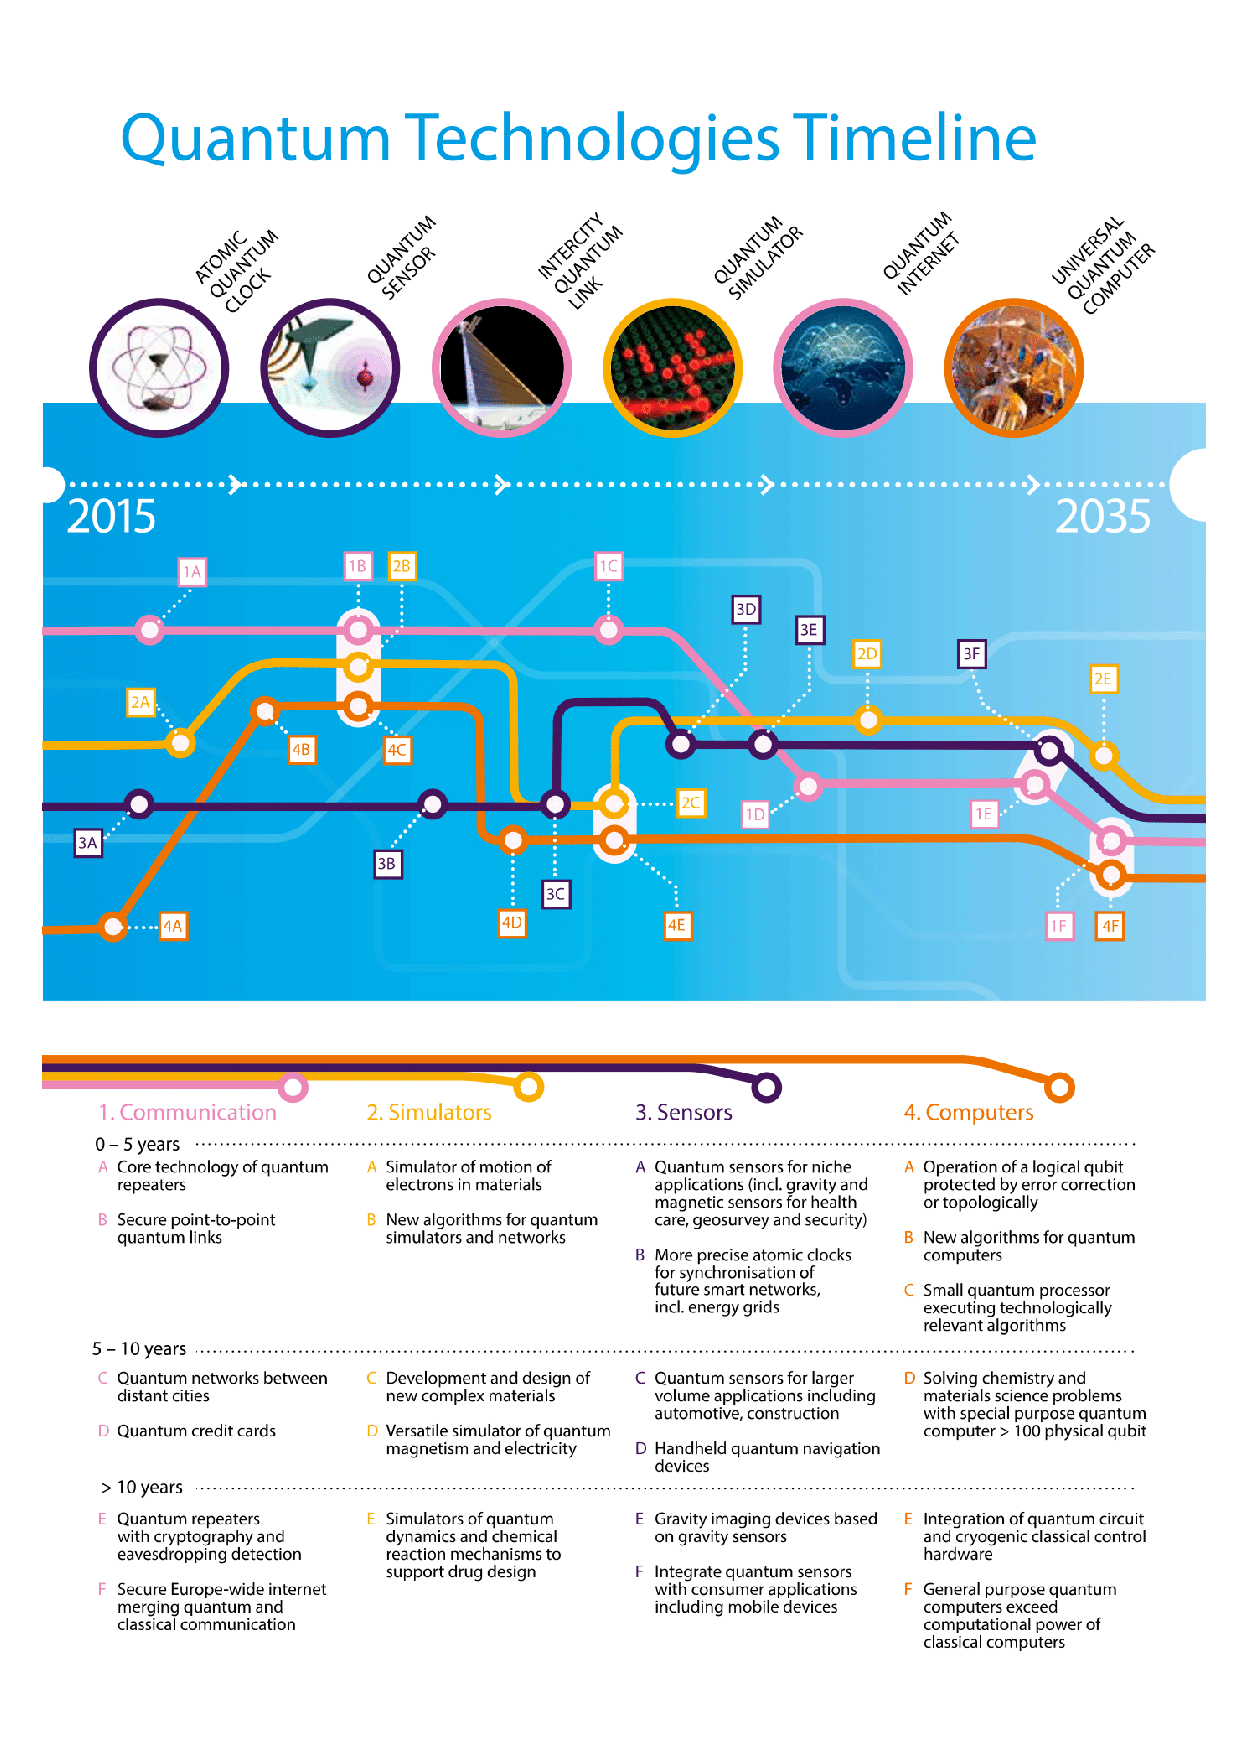
\includepdf{kep.pdf}
A kutatási, fejlesztési célokon felül egy igen fontos terület még az elméleti eredmények gyakorlatba ültetése, a mindennapi életet segítő piacképes alkalmazások létrehozása, aminek fő eszköze az ipar. Ennek a fontossága a Manifesto-ban is látszik hiszen a vezető kutatási szerepen túl megjelölt a legfontosabb cél egy növekvő és versenyképes európai iparnak kedvező körnezet kialakítása. A kvantumkommunikáció terén a technológia fejlődésével az elmúlt években a kutató intézeteken kívül szerencsére egyre több ipari szereplő is elkezdett foglalkozni, mind európában, mind világszerte, ami az egyre közeledő széleskörűbb gyakorlati alkalmazások elterjedését jósolhatja. Ezekről egy kis áttekintő: \\

\section*{Kvantumkommunikációval foglalkozó cégek}

Az Európában kvantum technológiához köthető vállalkozásokról található egy adatbázis a QUROPE oldalán: \url{http://qurope.eu/db/industries} . A kvantumkommunikációhoz valamilyen módon köthetó vállalkozások nagy része egyelőre főprofilként hagyományos optikával(pl.:Adva Optical Newtorking,ADVR,Corning) valamint hagyományos IT biztonsági megoldásokkal(pl.:Eleven Paths,Genua,Omnisec,Senetas) foglalkozik, konkrét kvantumos megvalósításokkal nem. A főprofilként kvantumos technológiákkal foglalkozó fiatalabb cégek viszont terjednek, ilyenek például az ID Quantique SA, QuTools, SeQureNet és SQR Technologies.\\
\underline{ID Quantique SA}  (\url{http://www.idquantique.com/}) 
\includegraphics[height=0.5cm, keepaspectratio]{idq.png}\\
Az ID Quantique SA egy svájci vállalat, az itt felsoroltak közül a legnagyobb múlttal rendelkező, 2001 óta foglalkozik QKD megvalósításokkal és kínál is megoldásokat a piac számára. A kulcsszétosztáson kívül, mára már kvantum véletlenszám generátorokkal is bővült a kínálata. A világon jelenleg működö QKD hálózatok közül több kiépítésében is szerepet vállalt(pl.: Svájci, Tokiói QKD hálózat)\\
\underline{QuTools} (\url{http://www.qutools.com/}) 
\includegraphics[height=0.5cm, keepaspectratio]{qutools.png}\\
A QuTools egy 2005-ben alapított német cég, különböző kvantumkommunikációs technológiákban használatos eszközökkel foglalkozik. Kínálatukban találhatók kvantumos fotondetektorok és generátorok, valamint véletlenszám generátorok is.\\
\underline{SeQureNet} (\url{https://www.sequrenet.com/}) 
\includegraphics[height=0.5cm, keepaspectratio]{sequrenet.png}\\
A SeQureNet egy 2008-ban alapított francia startup, CVQKD(Continuous Variable Quantum Key Distribution) megvalósítást kínál a piac számára, amibe beletartozik mind az ehhez tartozó hardver és a hozzá tartozó szoftver is.\\
\underline{SQR Technologies} (\url{http://www.sqrtech.com/}) 
\includegraphics[height=0.5cm, keepaspectratio]{sqr.png}\\
Az SQR Technologies 2010-ben alakult Belgiumban,jelenleg ultragyors véletlenszám generátorokat( ~4Gbps) kínálnak és fejlesztenek.\\

A célzottan kvantumkommunikációval foglalkozó vállalkozásokon kívül nagyobb ipari szereplők közül is vannak a témában erősebb érdekeltséggel rendelkezők Európában. Angliában a British Telecom és a Toshiba ottani kutatólaboratóriuma dolgozik kvantumkommunikciós technológiák megvalósításán.Rajtuk kívül ilyen még például az Atos akiknek van egy átfogóbb kvantumos programjuk, melyben a kvantumkommunikáción belül a kvantumkriptográfiai algoritmusok fejlesztése is szerepet kapott.A holland KPN a már korábban említett ID Quantique -val közösen pedig a hálózatán tesztelt QKD-t.\\
Az Európai szereplőkönt kívül természetesen világszerte egyre több vállalat foglalkozik kvantumkommunikációval, köztük már ismertebb nagyobb multú, akár multinaciónális cégek is. Az AT\&T és Caltech(California Institute of Technology) kvantumhálózatok fejlesztésén dolgozik, a Raytheon QKD megvalósítás után lehetséges kvantum ismétlő fejlesztésével foglalkozik, kvantum kriptográfia és kommunikáció szerepel a HP érdekeltségi listáján is, az SK Telecomnak is van már kvantumkommunikációs részlege, valamint Japánban a Tokiói QKD hálózatban együttműködő partnerek között ott van a NEC, Mitsubishi és NTT(Nippon Telegraph and Telephone), valamint a 2015-ös akkori QKD távolságrekord felállításában partner volt a Fujitsu is.\\
A főprofilban kvantumkommunikációval foglalkozó cégek közül a korábban már említetteken túl  piackész rendszererekkel rendelkezik az ISARA (aki kvantumos kutatásban együttműködik a Blackberryvel, szakterültetük a poszt-kvantum kriptográfia), MagiQ (kvantumkriptográfiai rendszer, összefonódott fotonpár forrás), NuCrypt (Összefonódott fotonpár forrás és detektor), QuantumCTek (QKD rendszerek, források, detektorok), Qubitekk (QKD rendszer), Quintessence Labs (véletlenszám generátor, biztonsági megoldások) és UQDevices (detektor). Ezeken a vállakozásokon felül vannak még egyelőre termék nélküli kutatás fejlesztéssel, valamint tanácsadással foglalkozók is. A Wikipédián a teljesség igénye nélkül található egy lista a témában érdekelt vállalatokról ami kiindulási alapként szolgálhat: \url{https://en.wikipedia.org/wiki/List_of_Companies_involved_in_Quantum_Computing_or_Communication}.




